\documentclass[11pt, oneside]{article}
\usepackage[margin=1in]{geometry}
\geometry{letterpaper}
\usepackage{booktabs}
\usepackage{hyperref}
\usepackage{enumitem}
\usepackage{float}
\usepackage{caption}
\usepackage{subcaption}
\usepackage[numbers]{natbib}
\usepackage{graphicx}
\usepackage{amssymb}
\usepackage{amsmath}
\usepackage{array}
\usepackage{longtable}
\usepackage{xcolor}
\usepackage{tabularx}
\usepackage{setspace}
\usepackage{tikz}
\usetikzlibrary{positioning,arrows.meta,fit,backgrounds}
\hypersetup{
    colorlinks=true,
    linkcolor=blue,
    citecolor=blue,
    urlcolor=blue
}
% Items that still need the author's own input are shown in red.
\newcommand{\todo}[1]{\textcolor{red}{\textbf{[#1]}}}
% Set to true to include the appendix (it comes after the references).
\newif\ifappendix
\appendixtrue
\captionsetup{font=small,labelfont=bf,skip=3pt}
\setlength{\textfloatsep}{8pt plus 2pt minus 2pt}
\setlength{\floatsep}{6pt plus 2pt minus 2pt}
\setlength{\intextsep}{6pt plus 2pt minus 2pt}
\setlength{\parskip}{0pt}

\title{CS781 Capstone Project:\\
In-House Legal Intelligence System}
\author{
    Nikhil N \\
    230697 \\
    {\tt nikhiln23@iitk.ac.in}\\
    Indian Institute of Technology Kanpur (IIT Kanpur)
}
\date{}
\begin{document}
\maketitle
\begin{abstract}
Law firms cannot send privileged case files to hosted language models, so we built a self-hosted legal NLP stack under a 50M--300M parameter cap, with no pretrained weights and Kaggle-class compute.
Phase~1 trains four decoder-only legal language models from scratch on a 4.5B-token Indian legal corpus (Acts, High Courts, Supreme Court, Tribunals) with a custom 50k byte-level BPE tokenizer: a grouped-query-attention (GQA) baseline of 138M parameters, a latent-attention/sparse-attention/MoE model of 222M, a GQA--RetNet hybrid of 165M, and a GQA/MHA mixture-of-experts model.
Phases~2--7 freeze these backbones and adapt them with hand-written LoRA, LoRMA, adapters and distillation to NER, rhetorical roles, judgment prediction, statute identification, summarization and case retrieval.
LoRMA beat LoRA in NER and rhetorical roles but lost elsewhere, and its permutation variant failed to train on the dense backbone.
Distillation never beat its teacher, a tenfold perplexity gap shrank to a two percent BERTScore gap, and BM25 matched our neural retriever.
\end{abstract}

% ============================================================
\section{Competition Result}
% ============================================================
\noindent
\textbf{Codabench username:} nikhiln23
\hfill
\textbf{Roll number:} 230697

\smallskip
\noindent
Table~\ref{tab:leaderboard} lists the best valid score we obtained in each phase. Entries in red could not be recovered from our logs and must be filled in from the leaderboard before submission.
\begin{table}[H]
\centering
\caption{Official phase scores and ranks. Rank and submission counts are read from Codabench at report freeze.}
\label{tab:leaderboard}
\small
\begin{tabular}{clcccc}
\toprule
Phase & Task & Primary metric & Value & Rank & Valid subs. \\
\midrule
1 & Legal LM Pretraining & BERTScore F1 & 0.8317 (M4) & 65 & 7 \\
2 & Legal NER & span F1 & 0.5929 (M4+LoRMA) & 17 & 7 \\
3 & Rhetorical role prediction & macro-F1 & 0.571 (M4+LoRMA) & 20 & 5 \\
4 & Court judgment prediction & macro-F1 & 0.6879 (M4+LoRA) & 86 & 6 \\
5 & Legal statute identification & macro-F1 & 0.3713 & 72 & 4 \\
6 & Abstractive summarization & BERTScore F1 & 0.8036 (M4+LoRA) & 122 & 4 \\
7 & Prior Case Retrieval & micro-F1@7 & 0.3237 (M4) & 93 & 4 \\
\bottomrule
\end{tabular}
\end{table}
\noindent
\textbf{Total valid Codabench submissions:} 37 \quad \textbf{Ranks recorded on:} 9 November 2026.
The minimum of four distinct submissions was met in every phase.

% ============================================================
\section{Introduction and Problem Description}
% ============================================================
A law firm's case files are privileged, so sending them to a hosted model is often not an option. The capstone therefore asks for an in-house legal intelligence system built from scratch: one foundation model trained by us, then adapted to six downstream tasks on Indian legal text. All data come from the single gated repository \texttt{Exploration-Lab/CS-781-Capstone}, and every task is scored on Codabench.

Phase~1 is autoregressive pretraining. Given a prompt of about 512 words, the model must continue it with exactly 128 whitespace-separated words that do not copy the prompt; the primary metric is BERTScore~F1 \cite{zhang2020bertscore}, with ROUGE-L \cite{lin2004rouge} and BLEU-4 \cite{papineni2002bleu} as secondary scores. Phase~2 is legal NER over 12 entity types with strict character-span matching. Phase~3 labels every sentence of a judgment with one of 13 rhetorical roles, in two domains (Corporate Law, CL, and Income Tax, IT), scored by macro-F1. Phase~4 predicts a binary court outcome from a full judgment (macro-F1). Phase~5 is multi-label statute identification over 99 statute ids. Phase~6 is abstractive summarization of long judgments, scored by BERTScore, and Phase~7 is prior-case retrieval: for each query case, return the relevant prior cases from a candidate pool, scored by micro-F1 at a cut-off of seven.

The constraints shaped almost every decision. The foundation had to have 50M--300M parameters, no pretrained language model or tokenizer was allowed, and no external legal corpus could be used. Compute was Kaggle's two T4 GPUs with a 30-hour budget per model and sessions that end after roughly ten to twelve hours. Judgments are far longer than any context we could afford, so long-document handling matters in four of the six downstream phases.

We investigated five questions. Which attention mechanism gives the best compact legal language model under a fixed budget? Does perplexity predict downstream quality? Which parameter-efficient method best adapts a frozen backbone, and does the answer depend on the task? Can distillation or ensembling recover the gap to the best single model? And how should long judgments be encoded: by truncation, head-and-tail views, or chunking? We built the full seven-phase pipeline end to end, with every adapter written by hand rather than taken from a library. We did not attempt full fine-tuning of the larger backbones except once in Phase~2, any external data, or human legal evaluation.

% ============================================================
\section{Data Analysis and Preprocessing}
% ============================================================
\subsection{Sources and official splits}
We used only \texttt{Exploration-Lab/CS-781-Capstone} and its official phase configurations. Phase~1 supplies a corpus of more than 4.5B tokens drawn from Acts, High Courts, Supreme Court judgments and Tribunals, plus a 1000-prompt test set. We held out whole documents (a \texttt{val\_tokens} file) for local generation scoring, separate from the per-source validation carve-out used for perplexity. Later phases use the official train, dev and test files. Phase~2 has fold-based validation (our fold~2 holds only 35 documents). Phase~3 has CL and IT domains, validated with five folds. Phase~4 has 2511 dev documents and 1517 test documents; Phase~5 has 42{,}178 train, 10{,}028 dev and 13{,}019 test documents; Phase~6 has about 100 test documents; Phase~7 has a query set that sits inside its own candidate pool.

\subsection{Corpus statistics that informed design}
We ran a standard audit notebook before every phase (cleaning, duplicate and leakage checks, length statistics, tokenization, folds). Four findings changed our designs.

\paragraph{Test leakage in Phase~4.} All 1517 test ids also appear in the labelled dev file with identical text. Only 994 of the 2511 dev documents were therefore safe to use for validation. We excluded the overlapping documents from training and validation, and the same exclusion rule was applied in Phases~5--7. Phase~5 showed the same effect on a smaller scale: 120 test documents repeat train or dev text, and on dev the 41 repeated documents had identical label sets to their train twins.

\paragraph{Where the signal sits.} In Phase~4 a TF-IDF probe over document sections showed that outcome-bearing text lives in the tail of the judgment, so every document is encoded as its first chunk plus its last three 1024-token chunks. In Phase~7, BM25 on the head and tail of each case reached an F1@7 of 0.32 on dev, against 0.19 on the full text, so each case is represented by its first and last chunk. In Phase~6 the opposite held: summary content is spread roughly uniformly over the document and summaries average about 984 tokens, so truncation would discard most of the target. An extractive oracle reached 0.736 unigram F1, which supported a chunk-then-merge strategy.

\paragraph{Imbalance and long tails.} Phase~5 has 99 statutes with 3.69 labels per document on average (maximum 31). The most frequent statute (id~5) appears in 11{,}522 training documents while the rarest appear fewer than 300 times (Figure~\ref{fig:statutes}); we treated the bottom 10\% by count (at most 334 documents, ten statutes) as rare. Phase~3 has a similar tail: PrecedentOverruled has three examples in total, and Dissent recall stayed near 0.09. Phase~2's weak labels were APP, RESP, WIT, AUTH and PREC.

\paragraph{Retrieval structure.} In Phase~7 every query appears in its own candidate pool, so its own id must be masked. The number of relevant cases per query ranges from 1 to over 90, and about 95\% of pool documents are gold for some query. Training queries form one giant connected group (510 of 816 queries share gold candidates), so cross-validation folds were unusable and the 118-query dev set served as validation.

\begin{figure}[t]
\centering
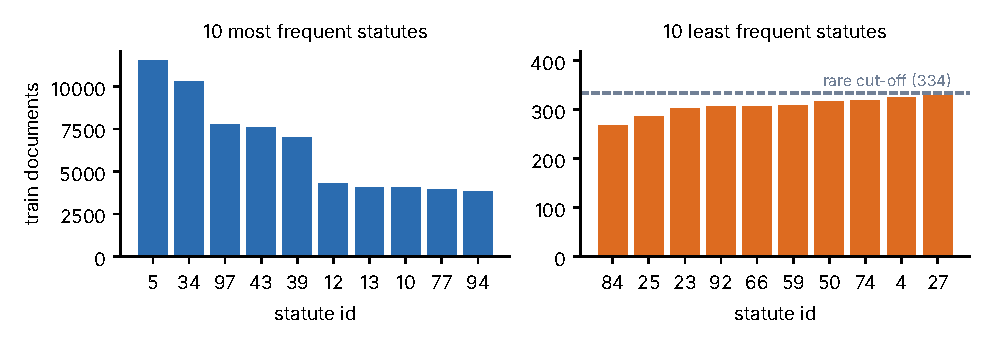
\includegraphics[width=0.85\linewidth]{figs/fig_statutes.pdf}
\caption{Phase~5 statute frequency in the training split, from our data-preparation log. The dashed line marks the cut-off below which a statute counts as rare.}
\label{fig:statutes}
\end{figure}

\subsection{Preprocessing}
\paragraph{Tokenization.} We trained a byte-level BPE tokenizer \cite{sennrich2016bpe} with a 50{,}000-entry vocabulary from scratch on the full corpus, in a CPU-only notebook, and shared it with all four models so that Phase~1 comparisons isolate the architecture. Because byte-level BPE can fold leading spaces into tokens, legal citations and section symbols are handled by the byte fallback rather than special rules. The tokenizer maps padding, separator and unknown to the same id~0; every downstream notebook therefore builds padding masks from sequence lengths and never from token ids.

\paragraph{Character offsets for NER.} Cleaning for Phase~2 is length-preserving, so gold offsets stay valid. Each document is encoded with the fast tokenizer's offset mapping, token offsets are trimmed of leading and trailing whitespace, and gold spans are checked and repaired against the text before tagging. Gold spans are converted to BIO tags (the longest span wins on overlap), and predicted tags are converted back to character spans through the same offsets. An oracle round trip (gold tags $\rightarrow$ spans $\rightarrow$ score) is run before any model is trained, which is how silent offset zeros are caught. Documents longer than the context are cut into overlapping windows, and each later window is prefixed with the document header so that party roles (APP/RESP) remain visible.

\paragraph{Long documents.} Phase~3 keeps the provided sentence lists and packs sentences into 1024-token windows with position features. Phase~4 uses first plus last three chunks. Phase~5 uses up to 32 chunks, which covers 99.8\% of documents, identically in training and inference. Phase~6 builds chunk-aligned targets by matching each summary sentence to the source chunk that best supports it, and keeps about half of the empty-target chunks so the model learns to say nothing. Phase~7 encodes each case as its head chunk and tail chunk with a shared policy for queries and candidates.

% ============================================================
\section{Approach and Model Evolution}\label{sec:approach}
% ============================================================
\subsection{Phase-1 foundation model}
We planned four substantially different models and trained all four on the same tokenized corpus. Figure~\ref{fig:system} shows the resulting system.

\begin{figure}[t]
\centering
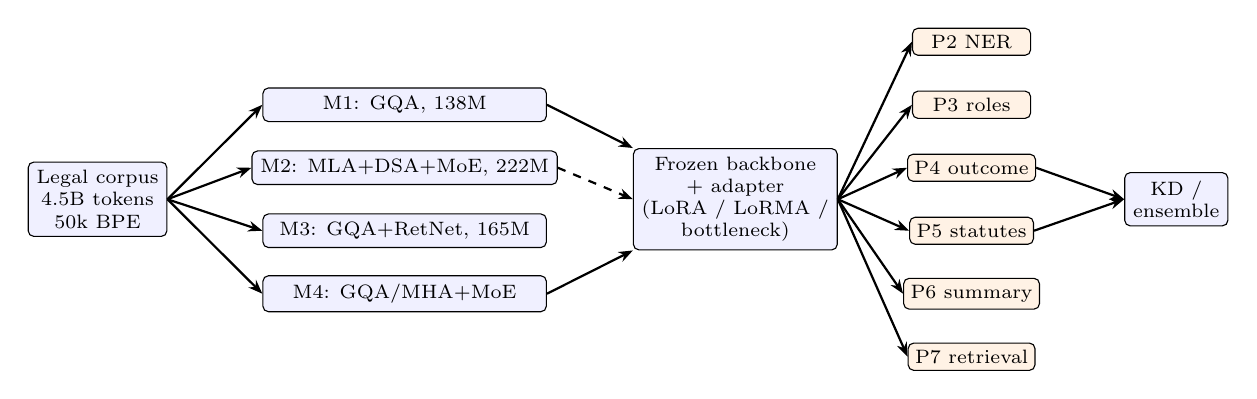
\begin{tikzpicture}[
  box/.style={draw, rounded corners=2pt, align=center, font=\scriptsize, inner sep=3pt, fill=blue!6},
  task/.style={draw, rounded corners=2pt, align=center, font=\scriptsize, inner sep=2.5pt, fill=orange!10, minimum width=15mm},
  arr/.style={-{Stealth[length=1.8mm]}, thick}]
\node[box] (data) at (0.9,0) {Legal corpus\\4.5B tokens\\50k BPE};
\node[box, minimum width=36mm] (m1) at (4.8,1.2) {M1: GQA, 138M};
\node[box, minimum width=36mm] (m2) at (4.8,0.4) {M2: MLA+DSA+MoE, 222M};
\node[box, minimum width=36mm] (m3) at (4.8,-0.4) {M3: GQA+RetNet, 165M};
\node[box, minimum width=36mm] (m4) at (4.8,-1.2) {M4: GQA/MHA+MoE};
\node[box] (peft) at (9.0,0) {Frozen backbone\\+ adapter\\(LoRA / LoRMA /\\bottleneck)};
\node[task] (t2) at (12.0,2.0) {P2 NER};
\node[task] (t3) at (12.0,1.2) {P3 roles};
\node[task] (t4) at (12.0,0.4) {P4 outcome};
\node[task] (t5) at (12.0,-0.4) {P5 statutes};
\node[task] (t6) at (12.0,-1.2) {P6 summary};
\node[task] (t7) at (12.0,-2.0) {P7 retrieval};
\node[box] (kd) at (14.6,0) {KD /\\ensemble};
\foreach \m in {m1,m2,m3,m4}{\draw[arr] (data.east) -- (\m.west);}
\draw[arr] (m1.east) -- (peft.north west);
\draw[arr] (m4.east) -- (peft.south west);
\draw[arr, dashed] (m2.east) -- (peft.west);
\foreach \t in {t2,t3,t4,t5,t6,t7}{\draw[arr] (peft.east) -- (\t.west);}
\draw[arr] (t4.east) -- (kd.west);
\draw[arr] (t5.east) -- (kd.west);
\end{tikzpicture}
\caption{System overview. Four decoder-only backbones are pretrained from scratch; Models~1 and~4 are frozen and adapted for Phases~2--7, each with its own task head, and results are combined by distillation or ensembling. Model~2 (dashed) was used only for a full fine-tune in Phase~2.}
\label{fig:system}
\end{figure}

\paragraph{Model 1 (GQA baseline).} Eight dense decoder layers with grouped-query attention \cite{ainslie2023gqa} (four key-value groups), rotary positions \cite{su2024roformer}, pre-normalization, a gated feed-forward block and FlashAttention kernels \cite{dao2022flashattention}. It has 138.25M parameters, a 1024-token context and a hidden size of 768, and was trained on 1.7B tokens. We verified the 50M--300M bound by counting parameters after construction. Its validation perplexity reached about 8.7.

\paragraph{Model 2 (MLA + sparse attention + MoE).} A DeepSeek-style stack \cite{deepseek2024v2} combining multi-head latent attention, a native-sparse-attention-style selector \cite{yuan2025nsa} and a six-expert mixture-of-experts feed-forward layer \cite{shazeer2017moe}, with 221.57M parameters. Its per-step cost was far higher, so it saw only about 0.95B tokens, and its final perplexity was 46.75. Building it surfaced four real bugs: a causality leak in chunk selection, a padding-boundary error, an uncounted quadratic cost in the indexer distillation loss (fixed by subsampling for a tenfold speed-up) and a dtype mismatch in the rotary tables under autocast. A warm-up value copied from Model~1 turned out to be 64\% of Model~2's much shorter run; we fixed it by resetting the schedule from the checkpoint without touching the weights.

\paragraph{Model 3 (GQA + RetNet).} Nine layers with GQA at layers 1, 5 and 9 and RetNet multi-scale retention \cite{sun2023retnet} elsewhere, a one-to-two ratio inspired by Jamba's hybrid recipe \cite{lieber2024jamba}, with a dense feed-forward block and 164.87M parameters. We proved the parallel, recurrent and chunkwise forms equivalent, which exposed a GroupNorm leak that mixed statistics across the whole sequence. Training repeatedly produced NaN losses, which we attributed to an fp16 overflow in the $QK^\top$ product. Retraining from scratch and a guard that stops on the first non-finite loss or gradient norm did not fix it (in the last logged run the loss jumped from 6.3 to 15.1 and the gradient norm became NaN at step 110 of 2{,}613), so Model~3 was never completed or scored.

\paragraph{Model 4 (GQA/MHA + MoE).} Nine layers with full multi-head attention at layers 1, 5 and 9 and GQA elsewhere, using Model~2's mixture-of-experts feed-forward module. MHA is GQA with as many key-value heads as query heads, so Models~1 and~4 differ mainly in the feed-forward design and layer mix, a limitation we accepted when we chose to drop the planned encoder--decoder model after the cost of Models~2 and~3.

\paragraph{Decoding.} Generation uses nucleus sampling \cite{holtzman2020nucleus} with top-$p=0.95$ and temperature 0.7, a ban on more than two identical consecutive words, a ban on repeated trigrams, incremental decoding that stops at 128 whitespace-separated words, and a check against copying the prompt verbatim.

\subsection{Transfer protocol (Phases 2--7)}
In every downstream phase the Phase-1 backbone stays frozen, and only an adapter plus a small task head train. We wrote all adapters ourselves, using only PyTorch primitives, and verified in each notebook that an adapter starts as the identity (outputs equal the Phase-1 model) and that base weights receive no gradient. The methods were LoRA \cite{hu2022lora} (rank 16, $\alpha$ of 16 or 32 by phase, on every linear layer in the blocks), LoRMA \cite{bihany2025lorma}, bottleneck adapters \cite{houlsby2019adapters}, and knowledge distillation \cite{hinton2015distilling}. LoRMA applies the low-rank factors multiplicatively to the frozen weight and restores rank either by cyclically rotating rows (\emph{perm}) or by adding the identity (\emph{plus}). On Model~4 the adapters wrap the attention projections and every routed and shared expert, while the router stays frozen; a start-up check confirms that each adapter kind is actually called under the routing logic and receives gradient. A tied-embedding bug (the output layer loading as random weights when it was not stored separately) was fixed in every notebook by re-tying it after loading.

\subsection{Task heads}
\paragraph{Phase 2, NER.} Token classification with a BiLSTM head, because a causal backbone only sees left context; decoding uses Viterbi over BIO tags, then same-name voting inside a document (a party named APP once should not be RESP elsewhere). A full fine-tune of Model~2 scored only 0.425 on fold~2 and was dropped.

\paragraph{Phase 3, rhetorical roles.} Sentences are packed into windows with relative-position and legal-cue features and classified by a BiGRU \cite{cho2014gru} head, trained jointly on CL and IT with inverse-square-root class weights, oversampling and a bias term tuned on out-of-fold predictions.

\paragraph{Phase 4, judgment prediction.} Each chunk is pooled from the backbone, a BiGRU runs over chunk vectors with attention pooling and a relative-position feature, and class-weighted cross-entropy trains the head; the decision threshold is tuned on out-of-fold macro-F1.

\paragraph{Phase 5, statute identification.} The same hierarchical head with 99 independent sigmoids, binary cross-entropy with a square-rooted positive weight, oversampling of rare statutes and one tuned threshold per statute.

\paragraph{Phase 6, summarization.} Decoder-only continuation with loss on the target only: each example is a source chunk, a separator, then that chunk's summary. At test time every chunk is summarized with greedy cached decoding and the pieces are joined in order. An extra ensemble stage selects, per document or per chunk, the candidate that agrees most with the other runs' candidates (minimum Bayes risk over ROUGE-1 and ROUGE-2), because averaging probabilities during decoding would cost the sum of all generation times.

\paragraph{Phase 7, retrieval.} A shared-weight bi-encoder with the adapter shared by queries and candidates, a multi-positive contrastive loss that never lets positives compete, hard negatives from BM25 and in-batch negatives (other queries' gold documents are natural hard negatives), and the query's own id masked in training and ranking. At inference the dev set chooses among plain cosine, centring, cross-query normalization (CSLS \cite{conneau2018csls} or dual softmax) and a BM25 hybrid \cite{robertson2009bm25}.

% ============================================================
\section{Experiments and Implementation Details}
% ============================================================
\subsection{Compute and training protocol}
All training ran on Kaggle: Phase-1 models on two T4 GPUs with a 30-hour budget each (fp16 autocast, data parallel), and downstream adapters on one T4. Phase-1 optimization used AdamW \cite{loshchilov2019adamw} with linear warm-up (derived as a fraction of total steps after the Model~2 incident), cosine decay, gradient clipping and dropout. Because sessions are killed after ten to twelve hours, every notebook saves checkpoints, stops cleanly at a time cap and resumes from an attached earlier output. Gradient checkpointing fixed T4 out-of-memory errors in Phase~5. A Model~1 summarization run took about 17 hours in practice, and a Model~1 judgment-prediction run took 105 minutes.

Table~\ref{tab:hparams} gives the main settings of the final runs. Learning rates and epoch counts per run are in Appendix~\ref{app:hp}.
\begin{table}[H]
\centering
\caption{Main settings of the final models. ``--'' means not applicable; LoRA / LoRMA settings are given in that order where they differ.}
\label{tab:hparams}
\scriptsize
\begin{tabular}{lcccccc}
\toprule
 & P1 & P2--3 & P4 & P5 & P6 & P7 \\
\midrule
Parameters (M) & 138--253 & frozen & frozen & frozen & frozen & frozen \\
Context / chunk & 1024 & window & 1024 & 1024 & 1024 & 1024 \\
Adapter & -- & LoRA/LoRMA & LoRA/LoRMA & LoRA/LoRMA & LoRA/LoRMA & LoRA/LoRMA \\
Rank, $\alpha$ & -- & 16,\,32 / 16,\,16 & 16,\,32 / 16,\,16 & 16,\,16 & 16,\,32 & 16,\,32 \\
Head & -- & BiLSTM / BiGRU & BiGRU+attn & BiGRU+attn & -- (LM) & shared encoder \\
Chunks per doc & -- & window & 4 & 32 & all & 2 \\
Decision rule & top-$p$ & Viterbi, bias & OOF threshold & per-label thr. & greedy & dev-chosen \\
\bottomrule
\end{tabular}
\end{table}

\subsection{Local evaluation}
We built held-out sets from public data in every phase: five stratified folds with out-of-fold predictions for Phases~3--5, the 994 leak-free dev documents for Phase~4, a 60-document fold for Phase~6, and dev queries for Phase~7. Out-of-fold scores, not single Codabench numbers, decided between variants, because several validation sets are tiny (35 NER documents, about 18 documents in a Phase~3 fold). We treated differences below about 0.01--0.02 (NER) and 0.03 (Phase~4) as noise. Local and Codabench scores agreed closely where the validation set was large: Phase~4 validated at 0.664 and scored 0.678, and Phase~5 Codabench scores ran about 0.015 below held-out estimates. Dev-tuned choices are slightly optimistic by construction.

\subsection{Ablations and controlled comparisons}
Each downstream phase changes one factor at a time: backbone (Model~1 versus Model~4), adapter (LoRA versus LoRMA) and, where run, training signal (hard labels versus distillation). Phase~7 adds an input-view ablation and a frozen-versus-adapted comparison; results follow.

% ============================================================
\section{Results}
% ============================================================
\subsection{Phase 1}
Table~\ref{tab:phase1} compares the three Phase-1 models that finished; Model~3 did not (Section~\ref{sec:approach}). Model~1 saw 1.79 times as many tokens as Model~2 and reached roughly a fifth of its perplexity, yet the BERTScore gap is only 2.3\% (Figure~\ref{fig:phase1}). Model~4 had the lowest perplexity (7.84) and the best BERTScore, but only 0.0012 above Model~1, which is within noise.
\begin{table}[H]
\centering
\caption{Phase~1 Codabench results on 1000 test prompts.}
\label{tab:phase1}
\small
\begin{tabular}{lcccccc}
\toprule
Model & Params & Tokens & Val. PPL & BERTScore F1 & ROUGE-L & BLEU-4 \\
\midrule
M1 GQA & 138.25M & 1.7B & 8.7 & 0.8305 & 0.184 & 0.0226 \\
M2 MLA+DSA+MoE & 221.57M & 0.95B & 46.75 & 0.8115 & 0.176 & 0.0160 \\
M4 GQA/MHA+MoE & 252.99M & $\sim$1.8B & 7.84 & \textbf{0.8317} & 0.186 & 0.0259 \\
\bottomrule
\end{tabular}
\end{table}

\subsection{Phases 2--7}
Table~\ref{tab:variants} gives Codabench primary metrics for every variant we scored; Figure~\ref{fig:peft} plots the adapter comparison for Phases~2 and~3, and Figure~\ref{fig:pcr} the Phase~7 dev results.
\begin{table}[H]
\centering
\caption{Primary metric per variant. M1/M4 = Model~1/4. Phase~5 values are out-of-fold macro-F1 (held out from tuning), not Codabench scores. Red entries need to be filled in from the leaderboard.}
\label{tab:variants}
\footnotesize
\begin{tabular}{clc|clc}
\toprule
Phase & Variant & Score & Phase & Variant & Score \\
\midrule
2 & M1 + LoRA & 0.5906 & 4 & M4 + LoRA & \textbf{0.6879} \\
2 & M4 + LoRA & 0.5661 & 4 & M1 + LoRA & 0.678 \\
2 & M4 + LoRMA (perm) & \textbf{0.5929} & 4 & other three (App.~A) & 0.669, 0.622, 0.600 \\
2 & KD (M4+LoRMA $\to$ M1) & 0.5798 & 4 & M1 + LoRMA-perm & 0.484 \\
2 & M2 full fine-tune (fold~2) & 0.425 & 5 & M1 + LoRA & 0.3864 \\
3 & M1 + LoRA & 0.518 & 5 & M4 + LoRA & 0.3811 \\
3 & M1 + LoRMA & 0.538 & 5 & M4 + LoRMA & 0.3733 \\
3 & M4 + LoRA & 0.537 & 5 & weighted ensemble & \textbf{0.3963} \\
3 & M4 + LoRMA & \textbf{0.571} & 6 & four runs, M1 and M4 & 0.8005--0.8036 \\
3 & M1 v2 (EMA, distillation) & 0.457 & 7 & M4 LoRA, LoRMA (test) & 0.3237, 0.3213 \\
 & & & 7 & M1 LoRA, LoRMA (test) & 0.3231, 0.3184 \\
 & & & 7 & ensemble, M1 KD (dev only) & 0.3613, 0.3480 \\
\bottomrule
\end{tabular}
\end{table}

\begin{figure}[t]
\centering
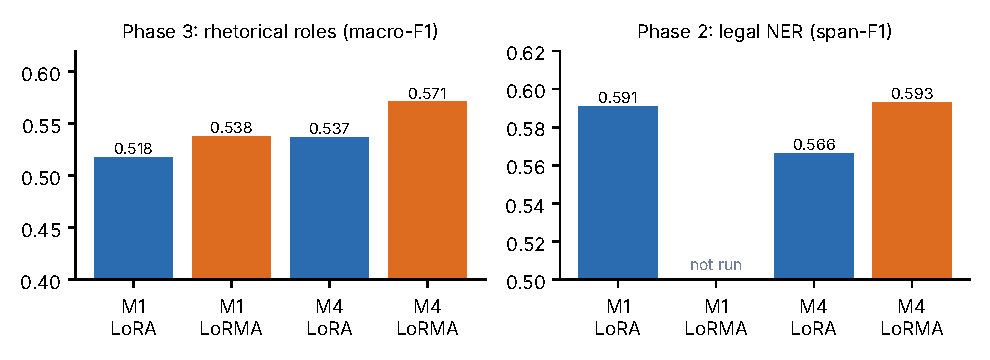
\includegraphics[width=0.85\linewidth]{figs/fig_peft.pdf}
\caption{LoRA (blue) versus LoRMA (orange) on the two backbones. LoRMA wins on both backbones in Phase~3 and on Model~4 in Phase~2.}
\label{fig:peft}
\end{figure}

\begin{figure}[t]
\centering
\begin{minipage}{0.48\linewidth}
\centering
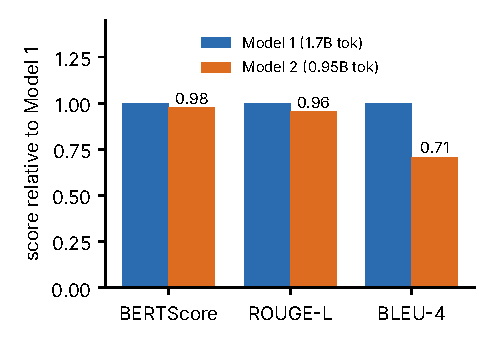
\includegraphics[width=0.88\linewidth]{figs/fig_phase1.pdf}
\captionof{figure}{Phase~1: Model~2's scores relative to Model~1.}
\label{fig:phase1}
\end{minipage}\hfill
\begin{minipage}{0.48\linewidth}
\centering
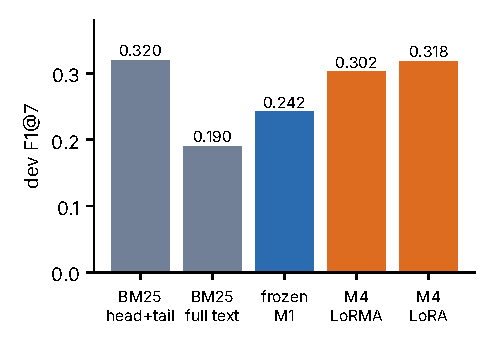
\includegraphics[width=0.88\linewidth]{figs/fig_pcr.pdf}
\captionof{figure}{Phase~7 dev F1@7: lexical baselines and neural runs.}
\label{fig:pcr}
\end{minipage}
\end{figure}

\paragraph{Which system won, and why.} In the phases where Model~4 was run, it won or tied (Phase~1: 0.8317 versus 0.8305): it beat Model~1 in Phase~3 by 0.033 with LoRMA and 0.019 with LoRA, and tied it in Phase~2 and Phase~5 within the noise band; in Phase~4 it led by 0.010 with LoRA (0.688) but trailed with LoRMA (0.600 versus 0.622 for LoRMA-plus on Model~1). We attribute this to the mixture-of-experts feed-forward layers: adapters on the routed and shared experts give the backbone more adaptable capacity than the dense layer for the same rank, whereas a frozen dense Model~1 can only be steered through its attention and one feed-forward block. Where the validation sets are small this is suggestive, not proven. LoRMA's advantage was phase-dependent: it won in Phases~2 and~3, lost to LoRA in Phase~5 (0.3733 versus 0.3811 on Model~4) and in Phase~7 dev (0.3024 versus 0.3180), and its perm variant failed outright on Model~1 in Phase~4 (0.484, below a trivial baseline), where a simulation at the real 768-dimensional hidden size showed it does not learn at any reasonable learning rate; switching to the plus variant fixed this. Averaging three Phase~5 runs raised held-out macro-F1 by only 0.010 over the best single run, which is inside the noise.

% ============================================================
\section{Error Analysis and Discussion}
% ============================================================
\subsection{Phase-wise failure modes}
\paragraph{Phase 1.} Model~1's Codabench file had a minimum prediction length of 74 words instead of 128. We believe this comes from the longest prompts (up to 911 tokens), where even the full 1024-token budget cannot hold 128 generated words; Model~4's minimum was 92 and Model~2's was 128. We did not confirm this prompt by prompt.

\paragraph{Phase 2.} Entity types tied to party role (APP, RESP) and to witnesses, authorities and precedents (WIT, AUTH, PREC) were the weakest, with recurring A.COUNSEL/R.COUNSEL confusion. A causal backbone cannot see which side a name belongs to until later in the document, which is why prefixing the header to every window and voting by name inside a document were the two corrections that targeted these labels. Under strict matching a one-token boundary slip scores as a complete miss.

\paragraph{Phase 3.} Rare roles failed first: PrecedentOverruled has three examples, and Dissent recall was 0.09 in a pooled out-of-fold check. The largest confusions, Ratio versus PrecedentReliedUpon and Fact versus ArgumentRespondent, depend on position in the whole judgment, while our head only sees 1024-token windows. Fold training loss fell to 0.35 while validation F1 peaked around epochs four to six, which signalled overfitting on a roughly 90-document pool.

\paragraph{Phase 4.} The 105-minute Model~1 run was undertrained: loss sat near 0.70 for 300 steps, validation F1 kept rising (0.558, 0.612, 0.641, 0.664) and the learning rate had already decayed to zero. About 28\% of documents are cut by the chunk limit, so a document whose outcome sits in a truncated middle section is predicted from the wrong evidence.

\paragraph{Phase 5.} Two Kaggle sessions hit the 10.5-hour cap mid-epoch, so at least one submitted run uses under-trained weights. Per-statute thresholds help rare labels but one global threshold would not, because macro-F1 weights a statute with 267 positives as much as one with 11{,}522. Frequent neighbouring sections co-occur heavily (for instance statutes 5 and 34 in 3596 training documents), which is why precision errors concentrate on near neighbours.

\paragraph{Phase 6.} Summaries average about 984 tokens with high variance. Chunk-wise generation can only be as good as the chunk-level alignment, and an oracle that copies the best source sentences reaches 0.736 unigram F1, so most of the remaining gap to references is selection rather than wording.

\paragraph{Phase 7.} Gold counts per query range from 1 to over 90 while the metric uses a fixed cut-off of seven, which caps achievable F1 on queries with many relevant cases. Both Model~4 adapters reached about 0.30--0.32 on dev, which is indistinguishable from BM25 on head and tail (0.32). Fusing neural scores with BM25 raised dev F1 to 0.348 for the Model~1 distillation student and 0.361 for the adapter ensemble, but these options were tuned on 118 queries and are optimistic; the student alone (0.301) stayed below its teachers (0.320).

\subsection{What the metrics do not measure}
BERTScore and ROUGE-L reward similarity to one hidden reference, not legal correctness: a fluent paragraph that drops the holding or cites the wrong section can score well. Strict span-F1 rewards offset perfection and gives no credit for correctly typing an entity whose boundary is off by one token. Macro-F1 over a handful of validation documents is dominated by rare classes. A real firm would need citation checks, entity linking to statute ids and lawyer review on top of these metrics.

\subsection{Limitations and next steps}
Compute shaped the study: Model~2 was trained on fewer tokens than Model~1 and Model~3 never finished, so the architecture comparison is confounded by budget; context was limited to 1024 tokens; and no external corpus or human evaluation was used. Phases were trained separately, so Phase~2 and~3 outputs were not used as features in Phase~4. Next experiments: retrain Models~2 and~3 at an equal 1.7B-token budget to separate architecture from data; train Phase~4 for three to four epochs at the higher adapter learning rate; add a document-level second-stage BiGRU over Phase~3 out-of-fold log-probabilities; and replace the fixed Phase~7 cut-off with a score-threshold rule fitted on dev.

\subsection{Surprising findings}
First, the perplexity gap between Models~1 and~2 is about five-fold at the end of training (roughly ten-fold at matched training fractions), yet Model~1 leads by only 2.3\% in BERTScore, 4.5\% in ROUGE-L and 41\% in BLEU-4 (relative to Model~2, on tiny absolute values). Second, the LoRMA permutation variant that was our best NER configuration failed to learn on the dense backbone, so a method's rank can reverse between tasks and backbones. Third, distillation never beat its teacher: in NER the student scored 0.5798 against the teacher's 0.5929, and the Phase~3 distillation variant fell to 0.457. Fourth, the 1517 test documents sitting inside the labelled dev file would have inflated any naive Phase~4 validation.

% ============================================================
\section{Conclusion}
% ============================================================
Three choices moved the metrics. The Model~4 mixture-of-experts backbone helped most in rhetorical roles; handling the data structure (header prefix and name voting in NER, tail-first chunking in judgment prediction, leak removal) mattered more than adapter choice; and per-label or per-class threshold tuning on out-of-fold predictions was the cheapest reliable gain (0.3748 to 0.3864 in Phase~5). Distillation and the permutation variant of LoRMA on the dense backbone did not help. The main lesson for training a compact legal model under a parameter and data lock is that downstream behaviour is only weakly tied to perplexity, so early downstream probes on a held-out slice are worth more than additional pretraining tokens. Code and notebooks are at \url{https://github.com/F1-N1ck/CS781-Legal-Intelligence-System-230697}.

\clearpage
% ============================================================
\section*{LLM Usage Declaration}
% ============================================================
\noindent
\textbf{Q1.} \todo{State the model(s) used, e.g.\ Claude (Anthropic), with version.}

\medskip
\noindent
\textbf{Q2.} \todo{Complete this table truthfully against your own workflow. Designing the architecture, hyperparameter search and writing the analysis and conclusions are not permitted uses.}
\begin{table}[H]
\centering
\small
\begin{tabular}{>{\raggedright\arraybackslash}p{4.6cm}|c|>{\raggedright\arraybackslash}p{7.2cm}}
\toprule
Part & Used LLM? & Purpose of using the LLM \\
\midrule
Understanding concepts / papers & \todo{Y/N} & \\
Ideation / brainstorming at a high level & \todo{Y/N} & \\
Debugging small ancillary snippets & \todo{Y/N} & \\
Plotting / visualization code & \todo{Y/N} & \\
Grammar / writing style of the report & \todo{Y/N} & \\
Report structure / section wording & \todo{Y/N} & \\
Designing the model architecture & \todo{Y/N} & \\
Hyperparameter search / tuning & \todo{Y/N} & \\
Analysis of results / conclusions & \todo{Y/N} & \\
Writing the core training / inference code & \todo{Y/N} & \\
Other (specify) & \todo{Y/N} & \\
\bottomrule
\end{tabular}
\end{table}

\noindent
\textbf{Q3.} Sources other than lecture slides and an LLM: the LoRMA paper \cite{bihany2025lorma}, the LoRA, GQA, RetNet, DeepSeek-V2, native sparse attention and Jamba papers cited above, the official dataset repository and the official Codabench evaluation scripts. \todo{Add any blogs, repositories or tutorials you used.}

\medskip
\noindent
\textbf{Q4.} \todo{Write 8--12 sentences in your own words about your own understanding, decisions, implementation, experiments and analysis. Failures you can name from the logs: LoRMA-perm did not learn on Model~1 in Phase~4 (0.484), distillation underperformed its teacher in Phases~2 and~3, Model~3 diverged to NaN from an fp16 overflow, and a copied warm-up value consumed 64\% of Model~2's run.}

\bibliographystyle{ieeetr}
\bibliography{references}

\ifappendix
\clearpage
\appendix
\section{Reproducibility and run inventory}
\label{app:hp}
Every phase follows the same shape: a data-preparation notebook (download from the gated repository, clean, audit, analyse, tokenize, build folds, write a helper module), then one notebook per backbone and adapter, then optional distillation and ensemble notebooks. Each notebook has a smoke-test switch, a session time cap with checkpoint resume, an identity check for the adapter, and writes \texttt{prediction.json}, \texttt{submission.zip} and a \texttt{run\_summary.json} with parameter counts, time and memory. Table~\ref{tab:inventory} lists the runs we completed, with the phase in which each was run.
\begin{table}[H]
\centering
\caption{Run inventory. ``Done'' means the run finished and was scored or evaluated; red marks runs whose outcome is not in our logs.}
\label{tab:inventory}
\small
\begin{tabularx}{\linewidth}{lX}
\toprule
Phase & Runs \\
\midrule
1 & M1 (1.7B tokens); M2 (0.95B tokens); M3 (not completed: NaN gradients); M4 \\
2 & M1+LoRA, M4+LoRA, M4+LoRMA-perm, M2 full fine-tune, KD (M4+LoRMA to M1), ensemble notebook \\
3 & M1+LoRA, M1+LoRMA, M4+LoRA, M4+LoRMA, M1 v2 (EMA and distillation) \\
4 & M4+LoRA 0.688 (selected), M1+LoRA 0.678, M1+LoRA on attention only 0.669 (one earlier submission cancelled), M1+LoRMA-plus 0.622, M4+LoRMA 0.600, M1+LoRMA-perm 0.484 (failed) \\
5 & M1+LoRA, M4+LoRA, M4+LoRMA-plus, weighted ensemble; M1+LoRMA not completed; KD notebook \\
6 & M4+LoRA 0.8036 (selected), M1+LoRA 0.8022, M1+LoRMA-perm 0.8017, M4+LoRMA-perm 0.8005; KD and the MBR ensemble were not among the four submissions \\
7 & M1 and M4 with LoRA and LoRMA-perm; KD student and ensemble (dev only, not submitted); frozen M1 baseline 0.2424 dev \\
\bottomrule
\end{tabularx}
\end{table}

\section{Additional hyperparameters and settings}
\begin{table}[H]
\centering
\caption{Per-phase adapter and training settings recovered from the notebooks.}
\small
\begin{tabularx}{\linewidth}{lX}
\toprule
Phase & Settings \\
\midrule
2 & Batch size 4; BiLSTM head; Viterbi decoding; header prefix on later windows; same-name voting chosen on fold~2 \\
3 & Five folds; inverse-square-root class weights; BiGRU head; EMA and per-class bias only in the abandoned v2 \\
4 & LoRA $r=16,\alpha=32$ on 7 linear layers; LoRMA-perm $r=16,\alpha=16$, LR $5\times10^{-4}$; chunks of 1024 with 128 overlap, at most 16; two epochs; pool~A of 10k documents, pool~B of 10k for distillation \\
5 & 32 chunks per document; BCE with square-root positive weight; per-statute thresholds on out-of-fold probabilities; gradient checkpointing; resume and eval-only modes \\
6 & LoRA on all 56 block linear layers, $r=16,\alpha=32$; model context 1024; two epochs; greedy cached decoding; half of empty-target chunks kept \\
7 & Shared-weight bi-encoder; multi-positive contrastive loss; BM25 top-100 hard negatives; cases encoded as head and tail chunks; dev-chosen scoring \\
\bottomrule
\end{tabularx}
\end{table}

\section{Phase-1 build log}
\begin{itemize}[leftmargin=*,itemsep=0pt]
\item \textbf{Model 1:} loss scaling bug from accepting \texttt{**kwargs} in \texttt{forward}; uninitialized rotary buffers after checkpoint reload; fp16 autocast not applied under data parallel.
\item \textbf{Model 2:} causality leak, padding-boundary error, quadratic indexer cost, dtype mismatch in rotary tables, warm-up sizing error.
\item \textbf{Model 3:} GroupNorm causal leak, memory-bandwidth bottleneck (solved by the chunkwise form), fp16 overflow in $QK^\top$, NaN guard added.
\item \textbf{Model 4:} reused tested modules from Models~1 and~2; warm-up computed as a fraction of total steps.
\end{itemize}
\fi
\end{document}
